\itodo{désassemblage parfait dans le cas sm}

Nous avons jusqu'à présent fait l'hypothèse \todo{todo} que les programmes analysés ne sont pas auto-modifiants.
Dans ce chapitre nous détaillons une approche d'analyse dynamique adaptée aux programmes auto-modifiants et ayant pour but de réduire l'analyse d'un programme auto-modifiant en l'analyse de plusieurs sous-ensembles non auto-modifiants du programme.
Cette approche est donnée par la littérature existante, en particulier par les travaux de thèse de Reynaud \cite{Reynaud2010} et Calvet \cite{Calvet2013}.

\section{Auto-modification et vagues}
Prenons le programme auto-modifiant donné à la figure \ref{fig:prg_asm_sm} et analysons une exécution de ses instructions de 1 à 5.
Deux instructions provoquent une auto-modification.
L'instruction 2 à l'adresse \adr{8048065} va provoquer une écriture à l'adresse pointée par la valeur de \eax\ incrémentée de 1, soit à l'adresse \adr{804806c}. Cette écriture modifie l'instruction 4 en \texttt{mov edi, 2}, codée sur les octets \texttt{bf 02 00 00 00}. De même l'instruction 3 modifie l'instruction 5 en \texttt{mov ebx, 2}, codée sur \texttt{bb 02 00 00 00}.
 
\begin{figure}
\begin{center}
\begin{tabular}[b]{|l|l|l|l|}
\hline
i & Adresse & Octets & Instruction\\ 
\hline
1 & 8048060  &  b8 6b 80 04 08         &  mov    eax, 0x8048076\\
2 & 8048065  &  66 c7 40 01 02 00      &  mov    [eax+1], 2 \\
3 & 804806b  &  66 c7 40 06 02 00      &  mov    [eax+6], 2 \\
4 & 8048076  &  bf 01 00 00 00         &  mov    edi, 1 \\
5 & 804807b  &  bb 01 00 00 00         &  mov    ebx, 1 \\
\hline
\end{tabular}
\end{center}
\caption{Programme auto-modifiant}
\label{fig:prg_asm_sm}
\end{figure}


Au vu de l'enchaînement des instructions, on peut construire trois représentations en mémoire des parties exécutables du programme.
La première correspond à la vision du programme lors de son chargement : la section .text est dans son état initial, donné en figure \ref{fig:prg_asm_sm}.
La seconde est celle après que la première modification du programme faite par l'instruction 2 et la troisième après la seconde modification effectuée par l'instruction 3.
En fait vu qu'aucune des adresses modifiées par la première instruction auto-modifiante n'est exécutée avant que la seconde modification ne soit faite, on peut regrouper les deux instructions auto-modifiantes et considérer que le programme n'a que deux représentations en mémoire : la représentation initiale et la représentation après que l'instruction 3 ait été exécutée. 
Beaucoup de logiciels protégés restaurent de grandes parties de code au démarrage : un grand nombre d'instructions sont modifiées sans que les instructions modifiées ne soient exécutées. 
Il nous paraît plus cohérent que toutes ces modifications soient réunies puisqu'elles correspondent à une étape lors de l'exécution du programme, l'étape suivante étant l'exécution d'une de ces instructions modifiées.

Dans ce découpage informel on appelle vague le désassemblage d'un instantané de la mémoire, pris à un instant donné. 
L'exécution d'un programme est alors caractérisée par une suite d'exécutions sur des vagues successives comme représenté en figure \ref{fig:vagues_visuel}. Les instructions qui sont présentes dans la trace sont colorées en rose tandis que le point d'entrée et la dernière instruction sont en orange et bleu clair, respectivement.
On passe d'une vague $k$ à la vague suivante $k+1$ lorsqu'une adresse mémoire écrite dans la vague $k$ est exécutée.
Ainsi dans une vague $k$, toutes les instructions exécutées ont été écrites au moins à la vague $k-1$. 
En ce sens chacune des vagues, prise indépendamment des autres, ne présente pas d'auto-modification.

Nous détaillerons par la suite ce qu'est une trace d'exécution pour l'analyse dynamique ainsi que la sémantique d'enchaînement des vagues.

\begin{figure}
 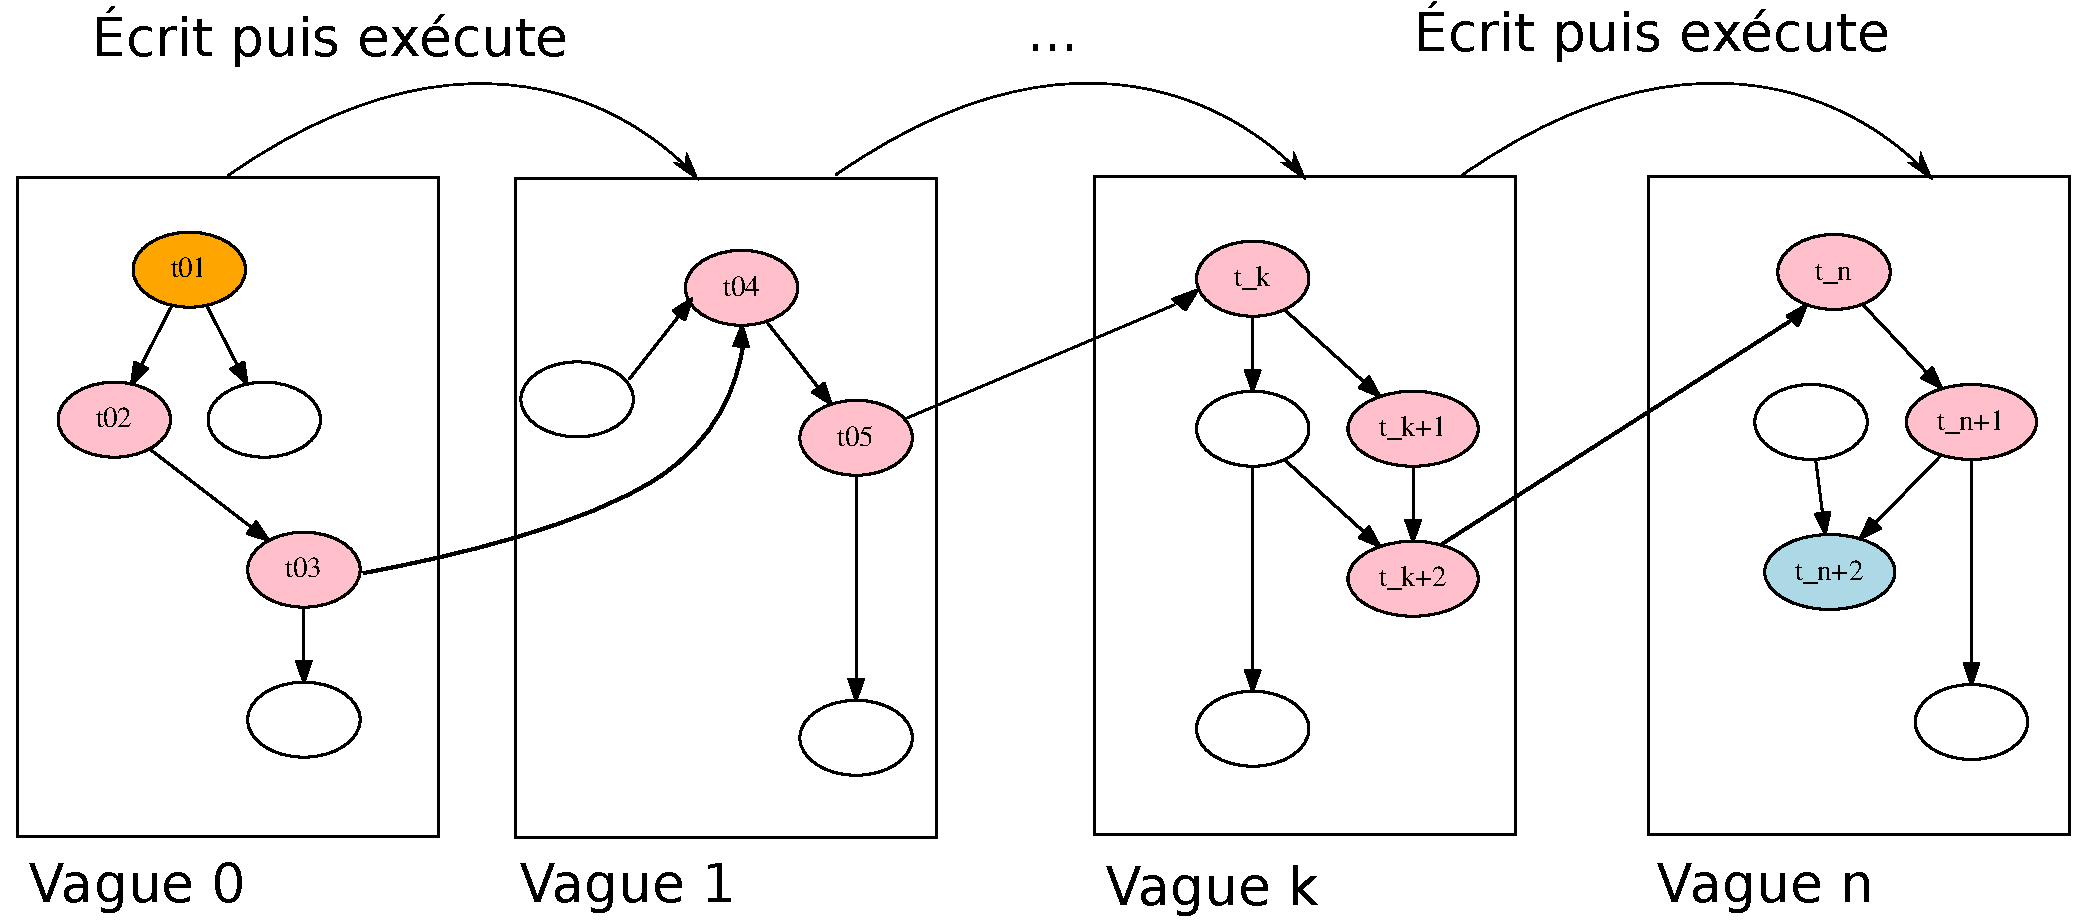
\includegraphics[width=1.0\textwidth]{supports/automodification/phases2_final.pdf}
 \caption{Vision informelle des vagues}
 \label{fig:vagues_visuel}
\end{figure}


\section{Revue de littérature}
La notion de vague présentée dans ce chapitre a été développée dans les thèse de Reynaud \cite{Reynaud2010} et Calvet \cite{Calvet2013}.
Elle est similaire à la notion de \emph{phase} présentée par Debray et Patel \cite{DP10} et utilisée pour automatiser la suppression de la protection d'un binaire. Le découpage d'une trace en phases est, chez eux, identique au découpage en vagues que l'on présente dans ce chapitre.
En particulier le programme auto-modifiant précédent (figure \ref{fig:prg_asm_sm}), exécuté, forme deux vagues : la vague initiale est le programme initial et la seconde, modifiée, est identique à l'exception des instructions 4 et 5 qui ont été modifiées en \texttt{mov edi, 2} et \texttt{mov ebx, 2} respectivement.
En général la suppression des protections se fait à l'aide d'une analyse dynamique et d'une image de la mémoire à un instant donné au cours de l'exécution. C'est cette image mémoire qui sera considérée comme étant le programme d'origine. La difficulté réside alors dans le choix de l'instant où prendre l'image mémoire : il s'agit souvent la dernière phase.

Preda, Giacobazzi, Debray, Coogan et Townsend \cite{PGDCT10} effectuent un découpage en phases mais chaque lecture d'une instruction écrite lors d'une vague précédente (pas uniquement lors de la phase en cours) provoque la création d'une nouvelle phase.
Avec l'exemple précédent, leur approche crée trois phases : la phase initiale, celle où uniquement l'instruction 4 a été modifiée, puis celle où les instructions 4 et 5 ont été modifiées.

\section{Trace, niveaux d'exécution et vagues}
Le programme exécuté a pour sources principales de données les registres et la mémoire constituée de la pile et du tas qui sont tous les deux adressables par des entiers. Une variable d'un programme est donc soit un registre du processeur soit une adresse mémoire, de même que défini dans la sémantique du langage intermédiaire défini au chapitre précédent (définition \ref{def:sem_conc_var}).

En utilisant la sémantique concrète précédemment définie on est capable, à partir d'un ensemble de valeurs initiales pour les registres et la mémoire, d'exécuter un programme sur cette entrée.
L'exécution d'un programme consiste en la définition d'un contexte d'exécution initial, l'évaluation sémantique de la première instruction dans ce contexte, puis l'évaluation de l'instruction suivante dans le contexte mis à jour, etc.

Nous définissons une instruction dynamique (définition \ref{def:ensembles_inst_dyn}) par son adresse, les adresses mémoires sur lesquelles elle est codée et l'instruction machine correspondant. Ces informations sont données par le décodage d'une instruction à l'adresse mémoire spécifiée dans un contexte donné. 

\begin{defi}
On note $D$ une instruction dynamique constituée des éléments suivants.
\begin{itemize}
 \item \da{D} l'adresse mémoire de l'instruction dynamique
 \item \dc{D} l'intervalle des adresses mémoire sur lequel $D$ est codée
 \item \di{D} l'instruction machine à l'adresse \da{D}
%  \item \dr{D_i} l'ensemble des variables sur lesquelles l'exécution de \di{D_i} provoque une lecture
%  \item \dw{D} l'ensemble des variables sur lesquelles l'exécution de \di{D} provoque une écriture
\end{itemize}
On définit l'opérateur \texttt{decode} qui associe à une adresse mémoire $a$ et un store $\Theta$ l'instruction dynamique $D=$\texttt{decode}$(a, \Theta)$ présente à l'adresse $a$.
\label{def:ensembles_inst_dyn}
\end{defi}

En pratique l'opération de désassemblage atomique définie au chapitre précédent nous donne ces informations. Pour l'assembleur \xq, une instruction est codée au maximum sur 15 octets.
Nous rappelons que nous notons, à tout instant durant l'exécution, $\Theta$ le store représentant l'état des variables (mémoire et registres) et $\BT$ l'ensemble des adresses mémoires.
Si on cherche à désassembler \telock\ à l'adresse \adr{0x01006e7a}, et qu'à l'adresse \adr{0x01006e7d} sont présents les octets suivant : $\Theta[0x01006e7d..0x01006e8b]=$ \texttt{eb ff c9 7f e6 8b c1 29 00 00 00 f3 aa 66 ab}, l'opérateur \texttt{decode} renvoie la première instruction dynamique D à cette adresse : il s'agit de l'instruction assembleur \di{D}=\texttt{jmp +1} (d'une taille de deux octets : \texttt{eb ff}) à l'adresse \da{D}=\adr{0x01006e7d}, codée sur l'intervalle d'adresses \dc{D}=[\adr{0x01006e7d}, \adr{0x01006e7e}].

Afin de pouvoir séparer la trace d'exécution selon le moment où chaque instruction a été écrite, nous définissons aussi, pour une instruction dynamique et un contexte d'exécution, l'ensemble des adresses mémoire sur lesquelles elle provoque une écriture (définition \ref{def:ensembles_inst_dyn_write}). Cette information est donnée par la sémantique concrète choisie. Avec la sémantique définie au chapitre précédent les seules instructions qui provoquent des écritures sont celles dont la liste d'instructions atomiques donnée par le désassemblage contiennent des assignations écrivant, par adressage direct ou indirect, à une adresse mémoire $m$. Si D est une instruction dynamique sémantiquement équivalente, dans le contexte $\Theta$, à l'enchaînement des instructions atomiques $d_1, ..., d_n$ alors \dww{\Theta}{D}=\dww{\Theta}{d_1}$\ \cup\ ...\ \cup\ $\dww{\Theta}{d_n} (propriété \ref{propri:eq_W_D_di}) avec
% \\
$$\mdww{\Theta}{d_i}=
\left\{
  \begin{array}{ll}
	  m &$ si $d_i=m\leftarrow g(x_1, ..., x_k)\ et\ m\in\BT
	\\\Theta(v) &$ si $d_i=[v]\leftarrow g(x_1, ..., x_k)\ et\ \Theta(v)\in\BT
	\\ \emptyset &$ sinon.$
  \end{array}
\right.
$$



\begin{defi}
Soit $D$ une instruction dynamique et $\Theta$ un store représentant l'état des variables (mémoire et registres). On note \dww{\Theta}{D} l'ensemble des adresses mémoire sur lesquelles l'exécution de $D$ provoque une écriture.
\label{def:ensembles_inst_dyn_write}
\end{defi}

\begin{propri}
Soit $D$ une instruction dynamique, $\Theta$ un store représentant l'état des variables (mémoire et registres) et $d_1, ..., d_n$ une suite d'instruction atomiques dans un langage intermédiaire telle que la suite d'instruction $d_1, ..., d_n$ dans le langage intermédiaire est sémantiquement équivalente à l'instruction assembleur \di{D}. On a :
$$\mdww{\Theta}{D}=\mdww{\Theta}{d_1,..., d_n}=\mdww{\Theta}{d_1}\ \cup\ ...\ \cup\ \mdww{\Theta}{d_n}.$$
\label{propri:eq_W_D_di}
\end{propri}

% \begin{defi}
% Nous définissons le niveau d'écriture d'une adresse mémoire comme un entier naturel et le store $W^M: \BT\rightarrow\BN$ associant à une adresse mémoire son niveau d'écriture.
% \label{def:store_mem}
% \end{defi}

Nous définissons plus formellement la notion de contexte d'exécution (définition \ref{def:contexte_exec}) comme la donnée d'un niveau d'exécution, d'un store contenant les valeurs de la mémoire et des registres et d'un store contenant les niveaux d'écriture courants de chaque adresse mémoire.

\begin{defi}
Un contexte d'exécution est la donnée d'un triplet $E=(X, \Theta, W^M)$ où
\begin{itemize}
 \item $X\in\BN$ est le niveau d'exécution du contexte
 \item $\Theta$ est le store des valeurs du contexte, associant une valeur à chaque registre et chaque adresse mémoire
 \item $W^M$ est le store des niveaux d'écriture du contexte, associant à chaque adresse mémoire un niveau d'écriture dans $\BN$
\end{itemize}
Une exécution d'un programme dont le point d'entrée est $ep$ est la donnée d'une suite finie de contextes d'exécution $E_0, E_1, ..., E_n$ tel que :
\begin{itemize}
 \item $X_0=1$, $\Theta_0[eip]=ep$ et $\forall m\in \BT, W_0^M[m\leftarrow 0]$
 \item En notant $D=$\texttt{decode}$(\Theta_i[eip], \Theta_i)$ l'instruction dynamique exécutée lors de la transition entre le contexte $E_i$ et $E_{i+1}$, on a :
    \begin{itemize}
     \item Le niveau d'écriture de $D$ est le niveau d'écriture maximum des octets qui la composent : $W_D=max(\{W^M[m],\ m\in\ $\dc{D_i}$\})$
     \item $X_{i+1}=max(X_i, W_D+1)$
     \item $\Theta_{i+1}$ est $\Theta_i$ mis à jour par l'évaluation sémantique de \di{D}
     \item $W_{i+1}^M=W_{i}^M$ sauf pour les adresses mémoire écrites par $D$: $\forall m\in\ $\dw{D}$,\ W_{i+1}^M[m\leftarrow X_i]$
    \end{itemize}
\end{itemize}
\label{def:contexte_exec}
\end{defi}

Une exécution consiste en une série de contextes d'exécution liés dont la transition est provoquée par l'évaluation sémantique de l'instruction pointée par le registre de compteur ordinal (noté en général \pc\ ou \eax\ en assembleur \xq), comme illustré par la figure suivante.

% \begin{figure}
\begin{center}
\scalebox{1}{
\begin{tikzpicture}[->,scale=1,>=stealth',thick]
\node[state, draw=none] (E0){$E_0$};
\node[state, draw=none, right=2cm of E0] (E1){$E_1$};
\node[state, draw=none, right=2cm of E1] (E2){$E_2$};
\node[state, draw=none, right=2cm of E2] (EP){$...$};
\node[state, draw=none, right=2cm of EP] (EN){$E_n$};
\draw (E0.east) -> node[above]{$D_1$} (E1.west);
\draw (E1.east) -> node[above]{$D_2$} (E2.west);
\draw (E2.east) -> node[above]{...} (EP.west);
\draw (EP.east) -> node[above]{$D_n$} (EN.west);
\end{tikzpicture}
}
\end{center}
% \caption{Enchaînement des contextes d'exécution et des instructions dynamiques}
% \label{fig:mem_process}
% \end{figure}


Nous avons donc, pour une exécution donnée, des niveaux d'exécution successifs $1, 2, ..., n$.
À chaque contexte d'exécution, toute adresse en mémoire $m$ a un niveau d'écriture $W^M[m]$ correspondant au dernier niveau d'exécution durant lequel une instruction a modifié la valeur à l'adresse $m$.
Une instruction $D$ a un niveau d'écriture $W_D$ qui est le niveau d'écriture le plus élevé parmi les adresses sur lesquelles elle est codée.
Lors d'une exécution le niveau d'exécution ainsi que le niveau d'écriture de chaque adresse mémoire sont croissants.



% \begin{defi}
% Nous définissons une trace d'exécution comme la donnée d'une suite $T=t_1, t_2, ..., t_n$ composée de triplets de la forme $t_i=(i, D_i, X_i)$ tels que
% \begin{itemize}
%  \item $D_i$ est la $i^{eme}$ instruction dynamique exécutée.
%  \item Avant l'exécution de l'instruction $D_i$, le niveau d'exécution est \texttt{$X_{i-1}$}.
%  \item Après l'exécution de l'instruction $D_i$, le niveau d'exécution est \texttt{$X_i$}.
% \end{itemize}
% \label{def:write_exec_levels}
% \end{defi}

\begin{defi}
Étant donnée une exécution d'un programme composée des contextes d'exécution $E_0, E_1, ..., E_n$ avec $E_i=(X_i, \Theta_i, W_i^M)$, on appelle trace d'exécution la suite $T=(t_1, t_2, ..., t_n)$ où $t_i=(i, X_{i-1}, D_{i-1})$ avec $D_{i-1}=$\texttt{decode}$(\Theta_{i-1}[eip], \Theta_{i-1})$
\label{def:trace}
\end{defi}

% \begin{propri}
%  Si le niveau d'exécution courant est $X$, le niveau d'exécution de l'instruction à exécuter $D_i$ est :\\
%  $X=max(X, W_D+1)$ avec $W_D=max(W^M[a],\ a\in\ $\dc{D_i}$)$.\\
%  Après l'exécution de $D_i$, les niveaux d'écriture dans la mémoire sont mis à jour de la manière suivante :\\
%  $\forall a\in$ \dw{D_i}, $W^M[a]=X$.
% \label{propri:niveau_exec}
% \end{propri}

En pratique une instruction $D$ écrite par une instruction ayant pour niveau d'exécution $k$ puis directement exécutée aura pour niveau d'écriture $W_D=k$ et pour niveau d'exécution $X=k+1$. On définit alors formellement instantané du niveau d'exécution $k$ selon la définition \ref{def:instantane} et une vague comme étant le désassemblage parfait de cet instantané (définition \ref{def:vagues}).
Une première vague est définie dès l'exécution de la première instruction du programme puis à chaque changement de niveau d'exécution une nouvelle vague est construite.
L'algorithme \ref{algo:analyse_dyn_vagues} permet d'exécuter un programme dynamiquement avec la sémantique concrète choisie tout en déterminant les niveaux d'exécution de d'écriture au fur et à mesure de l'exécution. La sortie de l'algorithme \ref{algo:analyse_dyn_vagues} est la trace d'exécution et la liste des vagues reconstruites.
\\

\begin{defi}
 Étant donnée une exécution d'un programme composée des contextes d'exécution $E_0, E_1, ..., E_n$ avec $E_i=(X_i, \Theta_i, W_i^M)$, on appelle instantané du niveau d'exécution $k$ l'état de la mémoire contenu dans $\Theta_j$ où $E_j$ est le premier contexte d'exécution dont le niveau d'exécution est $X_j=k$.
 On appelle point d'entrée et point de sortie de cet instantané respectivement $D_{in}=$\texttt{decode}$(\Theta_{j}[eip], \Theta_{j})$ et  $D_{out}=$\texttt{decode}$(\Theta_{l}[eip], \Theta_{l})$ où $E_l$ est le dernier contexte d'exécution dont le niveau d'exécution est $X_l=k$.
 \label{def:instantane}
\end{defi}

\begin{defi}
 Étant donnée une exécution d'un programme, on appelle vague $k$ le graphe de flot de contrôle parfait du programme représenté par l'instantané du niveau d'exécution $k$ muni de son point d'entrée.
 \label{def:vagues}
\end{defi}

Reprenons l'exemple du programme \sm\ précédent.
La figure \ref{fig:prg_asm_sm_trace} donne une trace d'exécution de ce programme en détaillant les informations sur chaque instruction dynamique ainsi que les niveaux d'écriture et d'exécution de chaque instruction.
Au départ toute la mémoire est dans son état d'origine et a pour niveau d'exécution 0. Lorsque l'instruction $D_1$ est exécutée, il n'y a pas eu d'auto-modification donc le niveau d'écriture est 0 et le niveau d'exécution est 1.
Les instructions $D_2$ et $D_3$ provoquent une auto-modification : les octets aux adresses \adr{0x8048077} et \adr{0x804807c} sont modifiés et leurs niveaux d'écriture deviennent donc le niveau d'exécution courant, soit 1.
Lorsque l'exécution atteint $D_4$, qui a été modifié, le niveau d'écriture est 1 donc le niveau d'exécution devient 2.
L'instruction suivante $D_5$ a également un niveau d'écriture de 1 donc le niveau d'exécution est inchangé.

Cette exécution est donc séparée en deux vagues : la vague initiale, $v_0$ dont l'instantané est l'état de la mémoire avant l'exécution de la première instruction et la vague $v_1$ contenant l'état de la mémoire juste après l'exécution de $D_3$ et avant l'exécution de la première instruction modifiée $D_4$.


% \begin{figure}
% \begin{center}
% \begin{tabular}[b]{|l|l|l|l|l|l|l|}
% \hline
% i & \da{D_i} & \dc{D_i} & \di{D_i} & \dw{D_i} & $W_i$ & $X_i$ \\
% \hline
% & 8048060  &  (...)         	        & Pile -> RWX &  & 0 & 1 \\ 
% 1 & 804807c  &  [804807c, 8048080]         &  mov    edi, 0x0 & edi & 0 & 1 \\
% 2 & 8048081  &  [8048081, 8048086]         &  mov    eax, 0x8048091 & eax & 0 & 1 \\
% 3 & 8048086  &  [8048086, 804808a]         &  mov    [eax], 0xeb & 0x8048091 & 0 & 1 \\
% 4 & 804808b  &  [804808b, 8048090]         &  mov    [eax+1], 0x7 & 0x8048092 & 0 & 1 \\
% 5 & 8048091  &  [8048091, 8048092]         &  jmp    80480a1 <edi3> &  & 1 & 2  \\
% 6 & 804809a  &  [804809a, 804809d]         &  mov    edi,0x2 & edi & 0 & 2\\
% 7 & 804809f  &  [804809f, 80480a0]         &  jmp    80480a8 <fin> &  & 0 & 2\\
%  & 80480a8  &  (...)		        &  Affiche edi &  & 0 & 2\\
%  & 80480c3  &  (...)		        &  Quitte &  & 0 & 2\\
% \hline
% \end{tabular}
% \end{center}
% \caption{Trace d'exécution du programme auto-modifiant de la figure \ref{fig:unevague_v0}}
% \label{fig:unevague_trace}
% \end{figure}

\begin{figure}
\begin{center}
\begin{tabular}[b]{|l|l|l|l|l|l|l|}
\hline
i & \da{D_i} & \dc{D_i} & \di{D_i} & \dw{D_i} & $W_i$ & $X_i$ \\
\hline
1 & 8048060  & [8048060, 8048064] & mov    eax, 0x8048076  &           & 0 & 1 \\
2 & 8048065  & [8048065, 804806a] & mov    [eax+1], 2      & 0x8048077 & 0 & 1 \\
3 & 804806b  & [804806b, 8048075] & mov    [eax+6], 2      & 0x804807c & 0 & 1 \\
4 & 8048076  & [8048076, 804807a] & mov    edi, 1          &           & 1 & 2 \\
5 & 804807b  & [804807b, 804807f] & mov    ebx, 1          &           & 1 & 2 \\
\hline
\end{tabular}
\end{center}
\caption{Trace d'exécution du programme auto-modifiant de la figure \ref{fig:prg_asm_sm}}
\label{fig:prg_asm_sm_trace}
\end{figure}

\begin{algorithm}[h] %or another one check
\caption{Mise à jour du niveau d'exécution d'une instruction}
\SetAlgoLined
\KwIn{La mémoire, l'opérateur de niveau d'écriture, une instruction dynamique et le niveau d'exécution courant}
\KwResult{Le niveau d'exécution courant mis à jour}
\SetKwProg{Fn}{}{}{}
\SetKwFunction{FRecurs}{MAJExecution}
\Fn(
){\FRecurs{M, $W^M$, D, X}}{
$W_D \leftarrow\ max(W^M[a],\ a\in\ $\dc{D}$)$\\
$X \leftarrow\ max(X,\ W_D+1)$ \\
\Return X
}
\label{algo:update_exec_level}
\end{algorithm}

\begin{algorithm}[h] %or another one check
\caption{Mise à jour des niveaux d'écriture lors de l'exécution d'une instruction}
\SetAlgoLined
\KwIn{La mémoire, l'opérateur de niveau d'écriture, une instruction dynamique et le niveau d'exécution courant}
\KwResult{L'opérateur de niveau d'écriture mis à jour}
\SetKwProg{Fn}{}{}{}
\SetKwFunction{FRecurs}{MAJEcriture}
\Fn(
){\FRecurs{M, $W^M$, D, X}}{
\For {$m\in\ $\dw{D}}{
  $W^M[m]\leftarrow\ X$
}
\Return $W^M$
}
\label{algo:update_write_level}
\end{algorithm}

\begin{algorithm}[H] %or another one check
\caption{Analyse dynamique avec calcul des vagues}
\SetAlgoLined
\KwIn{Les registres R et une mémoire M dans laquelle un programme a été chargé à son point d'entrée \texttt{ep}}
\KwResult{La trace des instructions dynamiques chacune associée à leur niveau d'exécution et les différentes vagues de la trace}
\SetKwProg{Fn}{}{}{}
\SetKwFunction{FRecurs}{analyseDynamique}
\Fn(
% \tcc*[h]{C : matrice des associations possibles, i : numéro du prochain sommet de P à associer, F : liste des couples d'associations déjà faites}
){\FRecurs{R, M, ep}}{
\For{$m\in M$}{
  $W^M[m]\leftarrow 0$\\
}
$(X, X_{-1}, i, T, instantanes, eip)\leftarrow (1, 0, 1, \emptyset, \emptyset, ep)$\\
% $X\leftarrow 1$\\
% $X_{-1}\leftarrow 0$\\
% $i\leftarrow 0$\\
% $T\leftarrow \emptyset$\\
% $vagues\leftarrow \emptyset$\\
% $eip\leftarrow ep$\\
\While {la fin du programme n'est pas atteinte}{
\tcc{Le programme est exécuté en prenant l'instruction suivante à l'adresse eip}
$D\leftarrow decode(eip, M)$\\
$X\leftarrow MAJExecution(M, W^M, D, X)$\\
\If {$X \ne X_{-1}$}{
  \tcc{Quand le niveau d'exécution change, on prend un instantané de la mémoire}
  $instantanes\leftarrow instantanes\cup \{(X_{-1}, M)\}$
}
$X_{-1} \leftarrow X$\\
~\\
\tcc{On met à jour le contexte à partir de l'instruction courante en l'évaluant sémantiquement}
$(eip, R, M)\leftarrow sem\_eval(eip, R, M)$\\
$W^M\leftarrow MAJEcriture(M, W^M, D, X)$\\
$T\leftarrow T\cup\{(i, X, D_i)\}$\\
$i\leftarrow i+1$\\
}
\Return T, instantanes
}
\label{algo:analyse_dyn_vagues}
\end{algorithm}

\begin{rem}
 Étant donné la définition croissante des vagues, une instruction dynamique peut-être exécutée non seulement plusieurs fois dans la même vague mais également être présente à des vagues différentes.
\end{rem}

\section{Désassemblage d'un programme \sm}
\subsection{Désassemblage parfait}
Nous avons précédemment défini le désassemblage parfait d'un programme \nsm\ comme la donnée de l'ensemble des adresses auxquelles des instructions peuvent être atteintes lors de l'exécution.
Dans le cas d'un programme \sm, cette définition n'est pas suffisante puisque l'instruction présente à une adresse dépend du contexte d'exécution et des éventuelles modifications qui ont été faites à cette adresse.

Nous considérons toujours que la donnée que l'analyste cherche à
déterminer et représenter est l'ensemble des exécution possibles du
programme : nous notons $E_T$ l'ensemble des traces d'exécution possibles.
En particulier une entrée spécifique provoque une exécution que nous observons sous la forme d'une trace.
Cette trace peut être découpée en niveaux d'exécution et chaque vague est le désassemblage parfait de l'instantané.

Le désassemblage, pris au sens de l'opération inverse de l'assemblage,
consiste à déterminer les adresses contenant des instructions, les
autres contenant des données.
Au sein d'une exécution les octets sur lesquelles une instruction ayant
un niveau d'exécution strictement supérieur à 1, c'est à dire que ces
octets ont été modifiés avant que l'instruction ne soit exécutée, ne
sont présents dans la représentation d'origine du programme qu'en temps
que données.
Ainsi le désassemblage parfait d'un programme \sm\ ne prend en compte
que les instructions exécutées avec un le niveau d'exécution 1
(proposition \ref{prop:desassemblage_parfait_sm}).

\begin{prop}
 Étant donné un programme P \sm\ et l'ensemble de ses traces d'exécution
$E_T$, le désassemblage parfait de P est l'ensemble des adresses où une
instruction de niveau d'exécution 1 est exécutée dans au moins une
trace, c'est à dire
 $\{a, \exists\ T\in E_T, \exists\ (i, X, D)\in T, X=1,\ $\da{D}$=a\}$.
\label{prop:desassemblage_parfait_sm}
\end{prop}


\subsection{Graphe de flot de contrôle parfait}
Le graphe de flot de contrôle ne peut plus se contenter de représenter
une instruction par son adresse puisque plusieurs instructions
différentes peuvent être présentes à la même adresse.
Le graphe de flot de contrôle parfait est alors le graphe dont les
sommets sont des couples $(a, I)$ où \adr{a} est une adresse et $I$ une
instruction assembleur. Il y a un arc entre deux sommets si le second
suit directement le premier dans une trace d'exécution (définition
\ref{def:cfg_parfait_sm}).

\begin{defi}
 Étant donné un programme \sm\ P et l'ensemble de ses traces d'exécution
$E_T$, le graphe de flot de contrôle parfait de P est le graphe orienté
$G=(V, E)$ tel que :
 \begin{itemize}
  \item $V=\{(a, I),  \exists\ T\in E_T, \exists\ (i, X, D)\in T,\
$\da{D}$=a,\ $\di{D}$=I\}$
  \item $((a_1, I_1), (a_2, I_2))\in E\ si\ et\ seulement\ si\ (a_1,
I_1)\ et\ (a_2, I_2)\ se\ suivent\ dans\ une\ trace\ : \exists T\in
E_T,\ i\in \BN, (i, X_1, D_1)\ et\ (i+1, X_2, D_2)\in T\ avec\
$\da{D_1}$=a_1,\ $\di{D_1}$=I_1,$~\da{D_2}$=a_2,\ $\di{D_2}$=I_2$.
 \end{itemize}
\label{def:cfg_parfait_sm}
\end{defi}

Le problème de cette définition d'un CFG pour un programme \sm\ est qu'%e souvent les vagues se suivent et ont peu de rapport les unes avec les autres.
elle ne permet pas de visualiser l'enchaînement des vagues et peut conduire à une interprêtation biaisée des exécutions possibles.

\paragraph{Exemple.}
Prenons le programme donné en figure \ref{fig:sm_asm} dont le graphe de flot de contrôle construit par analyse statique à l'aide d'un parcours récursif est en figure \ref{fig:sm_cfg_statique}.

\begin{figure}
\begin{center}
\subfigure[Code \sm]{
\begin{tabular}[b]{|l|l|l|l|}
\hline
Adresse & Octets & Instruction & Instruction écrite\\ 
\hline
 8048060 <debut>  &  31 ff             &  xor    edi,edi		& \\
 8048062  &  40                        &  inc    eax			& \\
 8048063  &  74 07                     &  je     804806c <si\_zero> 	& \\
 	  &			       &				& \\
 8048065  &  bf 02 00 00 00            &  mov    edi, 0x2 		& \\
 804806a  &  eb f4                     &  jmp    8048060 <debut> 	& \\
	  &			       &				& \\
 804806c <si\_zero> &  bf 01 00 00 00  &  mov    edi, 0x1 		& \\
 8048071  &  bb 60 80 04 08            &  mov    ebx, 0x8048060 	& \\
 8048076  &  66 c7 03 47 00            &  mov    [ebx], 0x47 		& inc edi\\
 804807b  &  66 c7 43 01 47 00         &  mov    [ebx+0x1], 0x47	& inc edi \\
 8048081  &  66 c7 43 03 c3 00         &  mov    [ebx+0x3], 0xc3	& ret \\
 8048087  &  eb d7                     &  jmp    8048060 <debut> 	& \\
\hline
\end{tabular}
\label{fig:sm_asm}
}
\subfigure[CFG par analyse statique et récursive]{
\includegraphics[width=0.8\textwidth]{supports/disas_sm/ex2_statique.pdf}
\label{fig:sm_cfg_statique}
}
\caption{Exemple d'un code \sm}
\label{fig:sm_exemple2}
\end{center}
\end{figure}

La branche du saut effectué à l'adresse \adr{0x8048063} dans le cas où \eax\ est différent de zéro revient vers le point d'entrée, incrémente \eax\ et passe à nouveau dans le saut conditionnel. Cette boucle provoquera à terme un dépassement d'entier sur la valeur \eax\ qui sera remise à zéro et l'autre branche du saut sera appelée.
Cette seconde branche a pour effet de modifier les instructions aux adresses \adr{0x8048060}, \adr{0x8048061} et \adr{0x8048063} pour y placer les instructions \texttt{inc edi}, \texttt{inc edi} et \texttt{ret} respectivement, puis de sauter sur l'adresse \adr{0x8048060}, provoquant l'exécution des instructions écrites ainsi que de l'instruction \texttt{inc eax}, non modifiée.

Ainsi toutes les exécutions possibles, paramétrées par la valeur initiale d'\eax, bouclent sur la branche conditionnelle un nombre fini, qui peut être nul, de fois et exécutent la seconde branche, qui met la valeur 1 dans \edi, provoque une auto-modification, incrémente \edi\ deux fois puis quitte la fonction. Dans toutes les exécutions possibles la valeur finale de \edi\ est toujours 3.

Le CFG parfait de ce programme est donné en figure \ref{fig:sm_cfg_parfait}. En raison du mélange des instructions à différents niveaux d'exécution, il n'est pas possible de distinguer les vagues d'exécution et un analyseur statique simple approxime la valeur de \edi\ à 2 ou 3.

\begin{figure}
\begin{center}
  \includegraphics[width=0.7\textwidth]{supports/disas_sm/ex2_parfait.pdf}
\end{center}
\caption{CFG parfait}
\label{fig:sm_cfg_parfait}
\end{figure}


Cette difficulté n'est pas intrinsèque aux programmes \sm\ et provient du fait même que le graphe de flot de contrôle est sur une surapproximation \todo{typo?} de l'ensemble des exécutions possibles. Il est cependant exacerbé dans le cas des programmes \sm\ puisque souvent les vagues successives n'ont que peu de code commun entre elles et il n'est pas cohérent de les mélanger dans le CFG.


\subsection{Graphe de flot de contrôle paramétré par une exécution}
Nous proposons une représentation du CFG basée sur une exécution particulière et son découpage en différents niveaux d'exécution.
Cette exécution consiste en une trace et un enchaînement d'instantanés de chaque niveau d'exécution.
Chaque instantané est pris comme un programme ayant pour point d'entrée la première instruction de la trace ayant le niveau d'exécution correspondant et un point de sortie étant la dernière instruction ayant ce même niveau d'exécution.
Nous appelons CFG paramétré par cette exécution l'union des CFG parfaits de chaque de ces instantanés dans lesquel les sommets sont caractérisés par le niveau d'exécution de l'instantané, une adresse et une instruction assembleur.
Un tel CFG pour le programme \sm\ précédent est donné en figure \ref{fig:sm_cfg_vagues} : l'exécution prise en compte est celle démarrant avec \eax=-2. La boucle directe est exécutée une fois, puis comme \eax=0, la partie auto-modifiante est activée.
\itodo{def formelle?}

% \begin{defi}
%  Étant donné un programme \sm\ P et une trace d'exécution $T$, le graphe de flot de contrôle de P paramétré par $T$ est $G=(V, E)$ tel que :
%  \begin{itemize}
%   \item $V=\{(a, I),  \exists\ T\in E_T, \exists\ (i, X, D)\in T,\
% $\da{D}$=a,\ $\di{D}$=I\}$
%   \item $((a_1, I_1), (a_2, I_2))\in E\ si\ et\ seulement\ si\ (a_1,
% I_1)\ et\ (a_2, I_2)\ se\ suivent\ dans\ une\ trace\ : \exists T\in
% E_T,\ i\in \BN, (i, X_1, D_1)\ et\ (i+1, X_2, D_2)\in T\ avec\
% $\da{D_1}$=a_1,\ $\di{D_1}$=I_1,$~\da{D_2}$=a_2,\ $\di{D_2}$=I_2$.
%  \end{itemize}
% \label{def:cfg_param_sm}
% \end{defi}

\begin{figure}
\begin{center}
  \includegraphics[width=0.7\textwidth]{supports/disas_sm/ex2_vagues.pdf}
\end{center}
\caption{CFG paramétré par l'exécution démarrant avec \eax=-2}
\label{fig:sm_cfg_vagues}
\end{figure}

Cette définition est particulièrement pertinente si quelle que soit l'exécution choisie les vagues d'exécution sont les même, comme c'est le cas dans l'exemple choisi ici.
Notre technique consiste donc à obtenir une exécution particulière d'un programme puis à augmenter la couverture de code à l'aide d'une analyse statique sur chaque instantané de l'exécution.

\subsection{État de l'art}

\section{Implémentations}
\todo[inline]{émulation VS instrumentation VS débogage}
\todo[inline]{BAP: \\
Jakstab: \\
TraceSurfer: (outil de daniel)\\
Renovo : \\
LLVM : (pk ne pas l'utiliser??) \\
Implem en C: \\
Xed : \\
}

Plusieurs choix s'offrent à qui cherche à implémenter un système d'analyse dynamique de binaire tels l'émulation, l'instrumentation et le débogage.

L'émulation consiste à lancer l'exécution dans un environnement d'exécution simulé, qui peut être un système d'exploitation complet comme c'est le cas avec BAP ou TEMU, le module d'analyse dynamique du projet BitBlaze \cite{bitblaze08}, basé sur l'émulateur QEMU \cite{QEMU05}.

On instrumente un binaire exécuté en y insérant, généralement au cours de son exécution, du code assembleur servant à son analyse. Intel développe PinTools \cite{pintools} pour l'analyse de programmes tournant sur leurs processeurs.

Enfin le débogage suit pas à pas l'exécution d'un programme en utilisant le drapeau de trappe (\emph{Trap Flag}), permettant de reprendre la main après chaque instruction du programme débogué afin d'examiner son environnement d'exécution.
\\

Le débogage comme l'instrumentation n'utilisent pas de langage intermédiaire tandis qu'un émulateur tel que BAP transcrit d'abord les instructions dans son langage intermédiaire pour les exécuter avec la sémantique concrète du langage intermédiaire.
L'émulation est donc intéressante parce qu'à aucun moment le programme analysé n'a un accès libre au système sur lequel il s'exécute.
La limitation est donc que les interactions du programme émulé avec le système d'exploitation visé sont restreintes.
En particulier les appels systèmes, qui ne sont pas transcrits par BAP, ne peuvent pas être émulés directement, rendant l'analyse très partielle.
Les approches nécessitant une exécution non restreinte sur le système sont alors réalisées au sein d'une machine virtuelle.

Une caractéristique cruciale d'un analyseur dynamique est qu'il doit être transparent : le programme analysé ne doit pas être capable de différencier son exécution dans l'analyseur de son exécution sur un système réel.
Cette transparence est en général partielle, que ce soit avec un émulateur, un débogueur ou une technique d'instrumentation.

L'instrumentation, par rapport au débogage, offre des performances temporelles d'exécution bien supérieures.
Pour ces raisons, nous nous sommes intéressés à l'émulation comme à l'instrumentation.
\\

L'émulation permet une analyse plus abstraite et nous avons développé un analyseur partiel de programmes auto-modifiants basé sur BAP.
L'instrumentation permet d'exécuter plus fidèlement le programme à analyser, nous avons donc principalement favorisé cette approche pour l'analyse de programmes malveillants. Nous avons choisi Pin qui, sans fournir de sémantique concrète pour l'assembleur, permet d'obtenir d'une instruction dynamique l'ensemble des adresses sur lesquelles elle écrit, comme souhaité à la définition \ref{def:ensembles_inst_dyn_write}.

\subsection{Émulation avec BAP}
Nous avons repris l'implémentation d'un émulateur pour programmes \sms\ basée sur BAP présentée au chapitre \ref{chap:semantique} et avons ajouté la séparation de la trace en plusieurs vagues d'exécution, selon l'algorithme \ref{algo:analyse_dyn_vagues}.

Cette implémentation donne le résultat attendu avec des programmes simples et qui n'utilisent pas d'appels système.
Sur l'exemple de programme \sm\ donné en début de chapitre, la sortie est la suivante.
L'exécution, de la première (\emph{pc: 1}) à la dernière instruction, est correctement découpée en vagues et les instructions correspondent à celles modifiées lors de l'exécution.

\begin{center}
\begin{verbatim}
Vague 1, pc: 1: addr 0x8048060 @asm "mov    eax, 0x8048071"
Vague 1, pc: 2: addr 0x8048065 @asm "movw   [eax+1], 2"
Vague 1, pc: 3: addr 0x804806b @asm "movw   [eax+6], 2"
Vague 2, pc: 4: addr 0x8048071 @asm "mov    edi, 2"
Vague 2, pc: 5: addr 0x8048076 @asm "mov    ebx, 2"
\end{verbatim}
\end{center}

Ne pouvant pas émuler des programmes utilisant des appels systèmes, nous avons laissé de coté cette approche pour une approche par instrumentation permettant l'analyse de programmes réels.


\subsection{Instrumentation avec Pin}

Pin est l'outil d'instrumentation développé par Intel pour ses processeurs \xq\ et \xs.
Il fournit un niveau d'information sémantique de niveau 2, donc suffisant pour suivre chaque instruction et connaître l'ensemble des adresses mémoire que l'instruction modifie. 
Nous avons à nouveau implémenté l'algorithme \ref{algo:analyse_dyn_vagues} sous la forme d'un PinTool : codé en C, il s'agit d'un programme définissant les actions à effectuer avant et après l'exécution de chaque instruction.
